\section{Introduction}

\begin{figure*}
  \centering
  \begin{subfigure}[t]{0.43\linewidth}
    \centering
  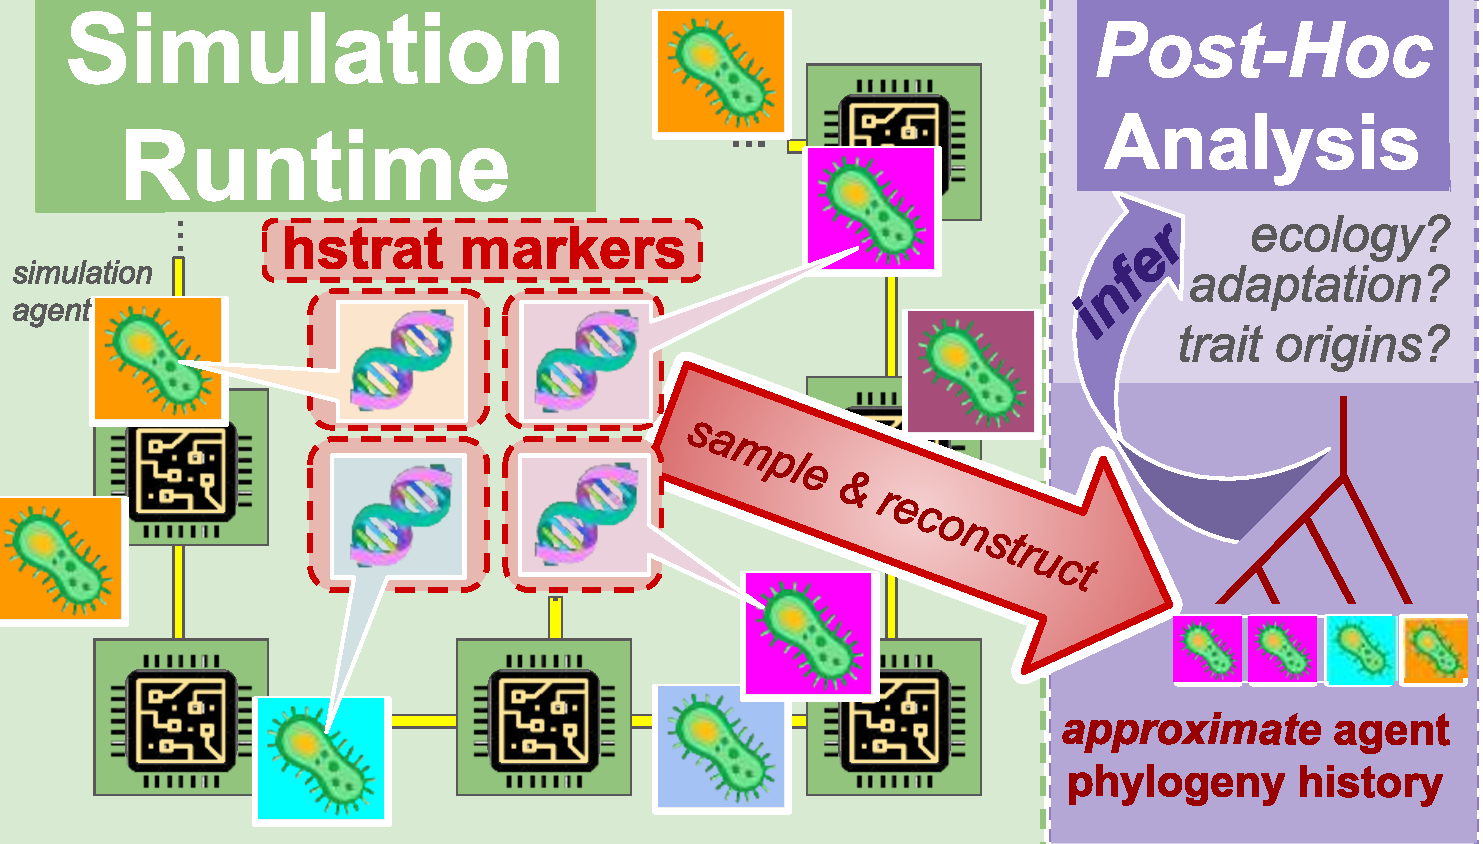
\includegraphics[width=\linewidth]{binder-wse-sketches/tex-access-proposal/img/runtime-posthoc-schematic}
    \caption{\footnotesize %
    hstrat markers help reconstruct phylogenies, which can tell evolutionary dynamics.
    }
    \label{fig:runtime-posthoc-schematic}
  \end{subfigure}
  \hspace{0.07\linewidth}
  \begin{subfigure}[t]{0.43\linewidth}
    \centering
  \includegraphics[width=\linewidth]{binder-wse-sketches/tex-access-proposal/img/async-ga-schematic}
    \caption{\footnotesize WSE island model evolutionary algorithm implementation.}
    \label{fig:async-ga-schematic}
  \end{subfigure}

\caption{%
\textbf{Methods for trackable distributed evolution simulation.}
\footnotesize
Subfigure \ref{fig:runtime-posthoc-schematic} shows use of hstrat markers to for reconstruct-based phylogenetic tracking of highly-distributed evolution simulations.
Subfigure \ref{fig:async-ga-schematic} summarizes asynchronous, callback-based approach to population exchange (``migration''') used to instantiate evolving populations across WSE PEs.
}
\label{fig:schematic}

\end{figure*}


% defining? fundamental?
A quintessential characteristic of computational artificial life experiments is the near total malleability of the simulacrum \citep{pattee1989simulations}.
Indeed, ability to explore arbitrary possibilities as-they-could-be is the core of artificial life's role as a tool for inquiry \citep{langton1997artificial}.
Such near-limitless freedom to realize arbitrary system configurations, however, can obscure an intrinsic limitation of most computational artificial life work: scale.

% Often, although not always, computational alife systems are designed for evaluation on a single CPU.
Take, for instance, the Avida platform, which instantiates populations of self-replicating computer programs for evolution experiments.
When running on a single CPU, this system can support about 20,000 generations per day, or about two hundred million individual replication cycles daily \citep{ofria2009artificial}.
By way of comparison, \textit{E. coli} populations within individual flasks of the Lenski Long-Term Evolution Experiment undergo only six doublings per day, meaning their generations take orders of magnitude longer than Avidians \citep{good2017dynamics}.
(In continuous culture, though, the rate can be c. 72 generations per day.)
Indeed, such capability for fast generational turnover has been a key motivation for using artificial life systems to study evolution.
However, the effective population size of flasks in the Long-Term Evolution Experiment is orders of magnitude larger than Avida's: 30 million vs. 10,000.
Consequently, these systems actually exhibit a similar number of replication events per day.
%With an effective population size of 30 million and around 6 doublings per day, about 180 million replication events elapse per day within each flask \citep{good2017dynamics}.
This pattern of dramatically faster generation times than those observed in nature and dramatically smaller populations largely generalizes across artificial life systems.
%Although Alife systems can typically observe generational cycles at orders-of-magnitude faster rates than their biological counterparts, population sizes are often limited and,
Of course, any such comparisons should also note profound discrepancies between the genetic, phenotypic, and environmental richness of biological organisms and alife models.
% Of course, such a comparison neglects profound incommensurabilities between Avidians and bacteria or yeast.
% Natural organisms have vastly more genetic content and phenotypic state, as well as more and more diverse interactions with the environment and with other cells.

% Adversely? Crucially? Conversely? Formidabbly? Aversely? Cumbrously?
Crucially, however, the scale of population size can greatly impact subjects of artificial life research, like transitions in individuality, ecological dynamics, and rare evolutionary innovations \citep{taylor2016open,dolson2021digital,taylor2019evolutionary}.
% Indeed, there is some evidence that limitations in scale are holding back \citep{CITEGEB}.
Cross-scale dynamics are also crucial to many key real-world challenges.
For example, in evolutionary epidemiology, interactions between within-host infection dynamics and population-level epidemiological patterns determine the evolutionary trajectory of the population \citep{schreiber2021cross}.
However, because capabilities of current Silicon-based processors are not expected to improve markedly in the forseeable future \citep{sutter2005free}, scale-up is necessary to progress on these key frontiers will demand many-processor computation.
Application of parallel and distributed computation, however, imposes compromises with respect to the convienence, flexibility, observability, interpretability, total reliability, and perfect replicability enjoyed under classical centralized, serial models of computation.
Encouragingly, these challenges are already implicit to much of biology; the productivity of research involving natrual organisms evidences that they are surmountable and even hints at strategies that can be used to solve them.
Here, we explore alignment of digital evolution to HPC accelerator hardware at the extreme cutting-edge of massively distributed computation, and use techniques inspired by those applied to natural organisms to mitigate limitations of distributed computation with respect to tracking phylogenies.

\subsection{Progress toward Scale-up in Artificial Life}

% effort
Achieving highly-scalable artificial life and digital evolution systems involves two distinct engineering considerations.
First, as with any high-performance scientific computing, careful design is required to appropriately divvy computation and communication workloads across available hardware.
% flexible/pliable/creative/abstract/representational/invites
% formulation
Second, given the exceptionally discretionary nature of artificial life modeling, we can intentionally tailor simulation semantics to suit underlying hardware capabilities.
% dichotomy
Ackley's ongoing work with the T2 Tile Project and ULAM exemplifies a strong synthesis of this engineering duality \citep{ackley2016ulam}.
At the level of simulation semantics, Ackley formulates update procedures in terms of local interactions between discrete, spatially situated particles.
This design provides for an efficient one-to-one mapping between simulation space and hardware components, minimizing requirements for intra-hardware connectivity and preventing global impacts from on-the-fly augmentations or reductions of available hardware.
The ULAM framework then ties into implementation-level infrastructure necessary to accomplish performant, best-effort lock/release of spatial event windows spanning bordering hardwares \citep{ackley2013movable}.
The Santa Fe Board project provided analogous infrastructure foundations for earlier work, coordinating efficient packet-framed, non-blocking communication between hardware tile elements \citep{livingcomputationSFBSanta}.
Ackley's work is distinguished, in fact, in dipping to a yet-lower level of abstraction and tackling design of bespoke, modular distributed processing hardware \citep{ackley2011homeostatic,ackley2023robust}.
% to engineer computational artificial life systems for scalability
% This work joins/builds on a longstanding chorus of interest in scale-up of artificial life, and already some exciting work in that domain.
% Of particular note is ADVOCACY/ARGUMENTATION Ackley has bespoke hardware \citep{ILLUMINAXMACHINA,ackley2023robust}.

% parallel and distributed
Several additional digital evolution projects have made notable headway in synthesizing artificial life models with sophisticated, scalable technical backing, achieving rich interactions among numerous parallelized simulation components.
Harding demonstrated large-scale cellular automota-based artificial development systems, achieved through GPU-parallelized instantiations of a genetic program  \citep{harding2007fast_ieee}.
Early work by Ray with Network Tierra used an island model to distribute digital organisms across federated servers, with migration handled according to the real-time latencies and topology of the underlying network \citep{ray1995proposal}.
More recently, Heinemann's continuation of the ALIEN project has leveraged GPU acceleration to achieve spectacularly elaborate simulations with rich interactions between numerous spatially-situated soft body agents \citep{heinemann2008artificial}.
Likewise, the Distributed Hierarchical Transitions in Individuality (DISHTINY) project has incorporated event-driven agent-agent interaction schemes amenable to best-effort, asynchronous interlocution \citep{moreno2022exploring,moreno2021conduit}.
GPU-first agent-based modeling (ABM) packages like Flame GPU also tackle this problem of hardware-simulacrum matching, albeit framed at a higher level of abstraction \citep{richmond2010high}.
Beyond alife, broader realms of application-oriented evolutionary computation have folded in with many-processor computation, most commonly through island-model and director-worker evaluation paradigms \citep{abdelhafez2019performance,cantu2001master}.

\subsection{Untapped Emerging Hardware}

In retrospect, connectionist artificial intelligence turns out to have been profoundly scale-dependent.
The utility and ubiquity of ANNs have exploded in tandem with torrential growth in training set sizes, parameter counts, and training FLOPs \citep{marcus2018deep}.
Recruitment of multi-GPU training for image classification, requisite particular accomodating adjustments to the underlying deep learning architecture, is commonly identified as the watershed moment to this transformation
 \citep{krizhevsky2012imagenet}.
Commerical investment in AI capabilies then set in motion a virtuous cycle of further-and-further-enabling hardware advances \citep{jouppi2017datacenter}.
Indeed, the scaling relationship between deep learning and training resources has itself become a major area of active study, with expectation for this virtuous cycle to continue through the forseeable future \citep{kaplan2020scaling}.

% The relationship between artificial life and scaling can be argued similar to that of connectionist artificial intelligence and scaling.
% except that artificial intelligence is a lot further along in this regard.
% % In important regards, the question of scale within artificial life parallels that within artificial intelligence,
% However, .
% The development of
% AlexNet united methodological innovations from the field (e.g., big data, dropout, ReLU) with GPU computing that enabled training of orders-of-magnitude-larger networks.
% In fact, .

% Spectacular advances achieved with artificial neural networks over the last decade illuminate one conceivable progression of events.
% As with digital evolution, artificial neural networks (ANNs) were traditionally understood as a versatile but auxiliary methodology --- both techniques have been described as ``the second best way to do almost anything'' \citep{miaoulis2008intelligent,eiben2015introduction}.

A major upshot of the deep learning race is emergence of a constellation of spectacularly capable next-generation compute accelerators \citep{zhang2016cambricon,emani2021accelerating,jia2019dissecting,medina2020habana}.
Although tailored expressly to deep learning workloads, these hardware platforms represent an exceptional opportunity to leapfrog progress on grand challenges in artificial life.
The emerging class of fabric-based accelerators, led by the 850,000 core Cerebras CS-2 Wafer Scale Engine (WSE) \citep{lauterbach2021path,lie2022cerebras}, holds particular promise as a vehicle for artificial life models.
This architecture interfaces multitudinous processor elements (PEs) in a physical lattice, with PEs executing independently with private on-chip memory and interacting locally through a network-like interface.

Our work here explores how such hardware might be recruited for large-scale digital evolution, demonstrating a genetic algorithm implementation tailored to the asynchronous, dataflow-oriented computing model of the CS-2 platform.
Indeed, rapid advances in the capability of accelerator devices, driven in particular by market demand for deep learning operations, is anticipated to play a key role in future advances in agent-based model capabilities \citep{perumalla2022computer}.
The very recent CS-3 chip announcement is fitting in this respect; among other spec enhancemments, it boosts clustering support to potentiallly thousands of constituent accelerators \citep{moore2024cerebras}.

% This will require changes and impose limitations to what is possible, artificial life.
% This is not an entirely unreasonable notion of a possible future of artificial life.

\subsection{Maintaining Observability}

% more is different More is different \citep{anderson1972more}.
% Likewise, progress of artificial life systems along a path, in the most ambitious framing, to indefinite scalability seems likely to unfold through incremental investments spurred by progressive scientific achievements.
% In tandem with more farsighted efforts, progress will also require prosaic leverage of existing, commercially-available parallel and distributed compute resources at circumstantially-feasible scales.
Orthogonalities between the fundamental structure and objectives of AI and artificial life methods will complicate any effort to requisition AI hardware for artificial life purposes.
In common use, deep learning operates as a black box medium \citep{loyola2019black} (but not always \citep{mahendran2015understanding}).
This paradigm de-emphasizes accessibility of inner state.
In contrast, artificial life more often functions as a tool for inquiry.
This goal emphasizes capability to observe and interpret underlying simulation state \citep{moreno2023toward,horgan1995complexity}.
(A similar argument holds for alife work driven by artistic objectives, as well.)
% Observability is even useful in goal-oriented evolutionary computation, where it can benefit diagnostics required to tune configuration to achieve good solution quality \citep{hernandez2022can}.

Unfortunately, scale complicates simulation observability.
% Scale transforms simulation into relentless data streams with
It is not uncommon for volume and velocity of data streams from contemporary simulation to outstrip hardware bandwidth and storage capacity \citep{osti_1770192}.
Intentional engineering effort will be required to ensure large-scale simulation retains utility in pursuing rigorous hypothesis-driven objectives.
% , and this problem is ubiquitous across simulation, observational, and experimental sciences
% Observability  and interpretability \citep{} will be key concerns, as will .

% To serve as a useful experimental platform, digital evolution simulations must be observable.
Here, we confront just a single aspect of simulation observability within distributed evolutionary simulation: phylogenetic history (i.e., evolutionary ancestry relationships).
Phylogenetic history plays a critical role in many evolution studies, across study domains and \textit{in vivo} and \textit{in silico} model systems alike \citep{faithConservationEvaluationPhylogenetic1992, STAMATAKIS2005phylogenetics,frenchHostPhylogenyShapes2023,kim2006discovery,lewinsohnStatedependentEvolutionaryModels2023a,lenski2003evolutionary}.
Phylogenetic analysis can trace the history of notable evolutionary events (e.g., extinctions, evolutionary innovations), but also characterize more general questions about the underlying mode and tempo of evolution \citep{moreno2023toward,hernandez2022can,shahbandegan2022untangling,lewinsohnStatedependentEvolutionaryModels2023a}.
Particularly notable, recent work has used comparison of observed phylogenies against those produced under differing simulation conditions to test hypotheses describing underlying dynamics within real-life evo-epidemiological systems \citep{giardina2017inference,voznica2022deep}.
Additionally, \textit{in silico}, phylogenetic information can even serve as a mechanism to guide evolution in application-oriented domains \citep{lalejini2024phylogeny,lalejini2024runtime,murphy2008simple,burke2003increased}.

\subsection{Decentralized Phylogenetic Tracking}

% Unfortunately, existing approaches to recording phylogenetic history from digital evolution simulations do not scale robustly.
In order to analyze the phylogenetic history of an evolving system, we must first collect it.
In existing artificial life work, a typical approach uses centralized tracking to maintain an exact, complete record comprising all parent-offspring relationships that have existed over the course of a simulation \citep{ray1992evolution,bohm2017mabe,de2012deap,garwood2019revosim,godin2019apoget,dolson2024phylotrackpy}.
Often, records of extinct lineages are pruned to prevent memory bloat \citep{moreno2024analysis}.
Although the direct-tracking approach is well suited to serial simulation or centralized controller-worker schemes, extreme sensitivity to missing data and runtime communication overheads impede scaling to highly distributed systems --- particularly those with lean memory capacity like the Cerebras WSE \citep{moreno2024analysis}.
To overcome this limitation, we have developed reconstruction-based approaches to phylogenetic tracking \textit{in silico} \citep{moreno2022hereditary}.
These approaches require no centralized data collection during simulation runtime; instead, they use \textit{post hoc} comparisons among end-state agent genomes to deduce approximate phylogenetic history --- akin to how DNA-based analyses tell how lineages of contemporary organisms relate in natural history.
Figure \ref{fig:runtime-posthoc-schematic} summarizes this reconstruction-based strategy.

Although analogous work with natural biosequences is notoriously challenging, uncertain, biased, and data-intensive \citep{neyman1971molecular,lemmon2013high},
recent development of hereditary stratigraphy algorithms provides a genetic annotation architecture explicitly designed for fast, accurate reconstruction requiring only small amounts of data.
% Work reported here uses just 96 bits of tracking information per agent genome.
Designed for attachment to underlying replicators as a neutral annotation (akin to noncoding DNA), it is a general-purpose technique potentially applicable across study domains \citep{liben2008tracing,cohen1987computer,friggeri2014rumor}.
In a stroke of convergent thinking, Ackley's recent work reports use of ``bar code'' annotations on his self replicators to achieve a measure of coarse-grained lineage tracing \citep{ackley2023robust}.
% Details on this methodology and our proposed approach to translate it to the WSE context is provided in Section \ref{sec:methods}.

\subsection{Contributions}

In this paper, we report new software and algorithms that harness the Cerebras Wafer Scale Engine to enable radically scaled-up agent-based evolution simulations while retaining key aspects of observability necessary to fully support hypothesis-driven computational experiments.
Implementation comprises two primary aspects:
\begin{enumerate}
  \item an asynchronous island-based genetic algorithm (GA) suited to the memory-scarce, highly-distributed, data-oriented WSE architecture, and
  \item a fundamental reformulation of hereditary stratigraphy's core storage and update procedures to achieve fast, simple, resource-lean annotations compatible with unconventional, resource-constrained accelerator and embedded hardware like the WSE.
\end{enumerate}

Both are implemented in Cerebras Software Language (CSL) and validated using Cerebras' SDK hardware emulator.
We use benchmark experiments to evaluate the runtime performance characteristics of the new hereditary stratigraphy algorithms in isolation and in the integrated context providing tracking-enabled support for the island-model GA.
In conjunction, we report emulated and on-device trials that validate phylogenetic reconstructions and demonstrate their suitability for inference of underlying evolutionary conditions.

Results from both experiments are promising.
We find that new surface-based algorithms greatly improve runtime performance.
Scaled-down emulator benchmarks and early on-hardware trials suggest potential for simple agent models --- with phylogenetic tracking enabled --- to achieve on the order of quadrillions of agent replication events a day at full wafer scale, with support for population sizes potentially reaching hundreds of millions.
Further, using proposed techniques, phylogenetic analyses of simulations spanning hundreds of thousands of PEs succeed in detecting differences in adaptive dynamics between alternate simulation conditions.

% \item WANT TO DO: we ran the async GA at full wafer scale on hardware with high/low selection pressure (tournament size 2 vs 8 ) and extracted  phylogenetic information; this phylogenetic information was sufficient to detect the difference in selection dynamics between the two runs.
% \end{itemize}

% Since the field's inception, artificial life has ridden a steady current of microprocessor innovation.
% As improvements in serial processing dried up around the turn of the century \citep{sutter2005free}, parallel and distributed became ascendant.
% As a result, it has become routine to dispatch independent instantiations of simulation runs across hardware units.
% In scientific contexts, this practice yields replicate datasets that provide statistical power to answer research questions \citep{dolson2017spatial}.
% In applied contexts, this practice yields many converged populations that can be scavenged for the best solutions overall \citep{hornby2006automated}.
% Another established practice is to use ``island models'' where individuals are transplanted between populations residing across distributed hardware \citep{gorges1990explicit}.
% Notably, asynchronous approaches are common and effective in these models \citep{abdelhafez2019performance}.

% Koza and collaborators’ genetic programming work with a 1,000-CPU Beowulf cluster typifies the island model approach \citep{bennett1999building}.
% In recent years, Sentient Technologies spearheaded evolutionary computation projects on an unprecedented computational scale, comprising over a million CPUs and capable of a peak performance of 9 petaflops \citep{miikkulainen2019evolving}.
% According to its proponents, the scale and scalability of this ``DarkCycle'' system was a key aspect of its conceptualization \citep{gilbert2015artificial}.
% Much of the assembled infrastructure was pieced together from heterogeneous providers and employed on a time-available basis \citep{blondeau2009distributed}.
% Unlike typical island models where selection occurs entirely independently on each CPU, this scheme transferred evaluation criteria between computational instances in addition to individual genomes \citep{hodjat2013distributed}.
% Sentient Technologies also notably exploited a large pool of hardware accelerators (e.g., 100 GPUs) in work evolving neural network architectures by performing each candidate architecture's costly model training and evaluation process \citep{miikkulainen2019evolving}.

% Existing parallel and distributed digital evolution systems typically minimize interaction between simulation components on disjoint hardware.
% Such independence facilitates simple and efficient implementation.
% This approach typically involves independent evaluation of sub-populations (i.e., island models) or individuals (i.e., primary-subordinate or controller-responder parallelism \citep{cantu2001master}).
% Cases where evaluation of a single individual are parallelized often involve data-parallel evaluation over a set of independent test cases, which are subsequently consolidated into a single fitness profile \citep{harding2007fast_springer, langdon2019continuous}.


% \section{Paths Forward}

% Implicit among much of the field, it seems, is an anticipation that order-of-magnitude changes in artificial life systems may unlock a qualitative sea change in simulation outcomes.
% This is not an entirely unreasonable notion of a possible future of artificial life.

% Spectacular advances achieved with artificial neural networks over the last decade illuminate one conceivable progression of events.
% As with digital evolution, artificial neural networks (ANNs) were traditionally understood as a versatile but auxiliary methodology --- both techniques have been described as ``the second best way to do almost anything'' \citep{miaoulis2008intelligent,eiben2015introduction}.
% However, the utility and ubiquity of ANNs has since increased dramatically \citep{marcus2018deep}.
% The development of AlexNet is widely considered pivotal to this transformation.
% AlexNet united methodological innovations from the field (such as big datasets, dropout, and ReLU) with GPU computing that enabled training of orders-of-magnitude-larger networks.
% In fact, some aspects of their deep learning architecture were expressly modified to accommodate multi-GPU training \citep{krizhevsky2012imagenet}.
% By adapting existing methodology to exploit commercially available hardware, AlexNet spurred the greater availability of compute resources to the research domain and eventually the introduction of custom hardware to expressly support deep learning \citep{jouppi2017datacenter}.

% Likewise, progress of artificial life systems along a path, in the most ambitious framing, to indefinite scalability seems likely to unfold through incremental investments spurred by progressive scientific achievements.
% To that end, observability \citep{moreno2023toward} and interpretability \citep{horgan1995complexity} will be key concerns, as will intentionally focuusing engineering effort to support hypothesis-driven objectives.
% In tandem with more farsighted efforts, progress will also require prosaic leverage of existing, commercially-available parallel and distributed compute resources at circumstantially-feasible scales.

% Such work should be made with an eye for contribution back to HPC.
% As noted earlier, the unique character of artificial life simulation suits it to serve at the tip of the spear in HPC evolution.
% High-performance computing hardware with transformative capabilities is coming to market right now, and some of it --- like the Cerebras wafer scale engine \citep{lauterbach2021path} --- is built explicitly for decentralized, asynchronous computation.
% Given ubiquity of deep net training and stencil-based numerical solvers in applications (CITE), programming for agent-based simulation can be of interest insofar as it flexes harware capabilities in unimagined ways.
% Effort to establish artificial life simulation as a flagship HPC application could be of mutual benefit.


% \section{Introduction} \label{sec:introduction}

% Agent-Based Modeling (ABM) has gained increasing adoption as a method to answer basic science questions and inform policy decisions.
% Despite a wide berth of application domains --- spanning sectors like spanning transportation infrastructure, public health, telecommunications, materials science and more --- much ABM work is unified by a common theme of interest in cross-scale dynamics.
% To provide such insight, ABM require sufficient scale to capture systems' emergent behaviors.
% Advances in high-performance computing (HPC) have already yielded paradigm-shifting improvements to the capabilities of ABM.
% However, across domains key questions still remain out of computational reach.

% Significant untapped potential for ABM scale-up has been identified in hardware-accelerator-enabled computation.
% Rapid advances in the capability of accelerator devices, driven in particular by market demand for deep learning operations, is anticipated to play a key role in future advances in ABM capabilities \citep{perumalla2022computer}.
% Within this category, the emerging class of fabric-based accelerators, most notably the recently-introduced 850,000 core Cerebras CS-2 Wafer Scale Engine (WSE) \citep{lauterbach2021path,lie2022cerebras}, is a particularly exciting --- and fairly uncharted, with applications to HPC workloads still in early days.
% This paradigm interfaces multitudinous processor elements (PEs) in a physical lattice, with PEs executing independently using individual on-chip memory and local PEs interacting through a network-like interface.

% \subsection{Objectives}

% This proposal establishes foundation for next-generation accelerator-enabled ABM computation by decentralized, approximate data export agent-based evolutionary simulation.
% In particular, we will evaluate asynchronous approaches for ABM migration/interaction on the WSE architecture to power agent-based evolution simulations, incorporating cutting-edge methods for distributed approximate phylogenetic (i.e., ancestry tree) tracking.

% Proposed work advances two technical objectives:
% \begin{enumerate}
% \item to evaluate and demonstrate new approaches for phylogenetic tracking in a massively-distributed, resource-constrained setting,
% \item to test the scalability of desynchronized agent migration procedures on WSE hardware,
% \end{enumerate}

% These technical capabilities will unlock capability to investigate a broad array of science questions.
% In this proposal, we focus on one science objective:
% \begin{enumerate}
% \item to evaluate how phylogenetic structure scales across orders-of-magnitude population sizes, and the extent to which commonly used phylogeny structure metrics are scale-invariant or scale-sensitive.
% \end{enumerate}

% Proposed work falls within the domain of agent-based evolution modeling, and uses it to explores phylogenetics-related inquiry by leveraging Cerebras WSE hardware.
% Our dual technical objectives constitute significant advancement of methodological capabilities within digital evolution, and our project will directly address fundamental open questions within the domain of phylogenetic theory.
% However, findings and methodologies will also generalize to other ABM domains beyond evolutionary simulation and to broader classes of highly-distributed HPC architectures.

% \subsection{Agent-based Evolution Simulation}

% Evolutionary processes do not confine to matters of natural history.
% Rather, evolutionary processes pervade our contemporary, everyday world.
% Key societal challenges root in evolving systems: antibiotic resistance, epidemiology, conservation biology, and oncology among others.  % citations?
% Evolutionary biology provides the fundamental foothold to efforts to address these problems \citep{aktipis2013evolutionary}.

% Mathematical and computational modeling complements natural history field work and benchtop evolution experiments as a crucial third leg to stand evolutionary inquiry.
% Simulation-based approaches provide key capabilities complementary to work with natural systems: complete observability, arbitrary manipulability, and rapid generational turnover.
% Within this context, agent-based simulation plays an important connective role between natural systems and abstracted, aggregate-based mathematical and numerical models.
% Agent-based approaches instantiate \textit{bona fide} evolutionary processes that track populations of virtual genomes subject to mutation, heredity, and selection \citep{pennock2007models}.
% This characteristic incorporates some of the critical complications and subtleties characteristic of natural systems --- e.g., arbitrary agent behavior, sophisticated agent-agent interactions, complex genotype-phenotype maps, albeit at significantly reduced scope and sophistication.

% Indeed, agent-based evolution approaches have provided means for fruitful investigation of wide-ranging hypotheses, including evolution of evolvability \citep{wilke2001evolution}, host-parasite co-evolution \citep{zaman2014coevolution}, evolution of complex traits \citep{lenski2003evolutionary}.

% Ambitious work advancing the field increasingly targets large cross-scale questions, including major transitions in evolution (e.g., multicellularity and symbiosis) \citep{goldsby2020major,vostinar2021symbiosis} and open-ended evolution (e.g., long-term trajectories of complex ecosystems with strong biotic selection) \citep{stanley2019open,taylor2016open}.
% Progress on these fronts demands computational substrate for orders-of-magnitude larger simulation scale than tractable today \citep{moreno2022exploring,channon2019maximum}.

% %as well as scenarios where replicating entities like cultural artifacts or computer viruses.
% % At the frontiers of evolutionary computation, there is in particular growing interest in the question of ``open-ended evolution'' \citep{}.
% % This refers to the problem of the inability to recreate the ongoing generation of novelty, complexity, and adaptation within the natural world.

% \subsection{HPC and Agent-based Evolution}
% % opportunity


% % Evolutionary questions often explicitly span scopes, with key areas of inquiry including ecologies of interacting populations and assembly of individuals into multicellular organisms and eusocial colonies \citep{morenoDISHTINYDOTO, citephageDOTO}.
% Researchers using agent-based evolution recognize HPC as critical to the future of the field \citep{ackley2016indefinite}.
% Indeed, the field has played host to notable boundary-pushing approaches to computing at the frontiers of computing hardware and modalities such as best-effort computing, reservoir computing, global-scale time-available computing, and modular tile-based computing in addition to more traditional cluster and GPU-oriented approaches \citep{moreno2021conduit,ackley2020best,ackley2023robust,heinemann2008artificial,miikkulainen2024evolving}.
% The diversity and, in cases, novelty of HPC within evolutionary simulation stems in large part from unique properties largely distinct from other HPC application domains.

% Given its inherent underlying stochastic nature and the stabilizing influence of adaptive selection, evolutionary simulation can often tolerate significant arbitrary asynchronicity or even entirely lost simulation components (e.g., dropped messages, crashed nodes, etc.).
% Likewise, digital evolution is typically amenable to locality restrictions of computation due to the inherent spatial structure of natural systems we are seeking to model.
% % In particular, massively-distributed, spatial computing being directly highlighted to be of particular interest \citep{ackleyDOTO}.
% Because agent behavior evolves over time, the influence of population-level drift and adaptive change can inject extreme heterogeneity to the computational workload profile of evolutionary simulation over time and simulation space.
% Finally, emerging directions have begun to tilt implementation towards more challenging communication-intensive qualities.
% The largely-decoupled nature of classic approaches within evolutionary computation like island models or controller/worker schemes  \citep{bennett1999building,cantu2001master} no longer suffice to realize the dynamic, communication-intensive interaction characteristic of major transitions and open-ended evolution \citep{moreno2022engineering}.

% These distinctive properties, position agent-based evolution as a potentially valuable testbed for HPC innovation and leadership.
% There is reason to expect a highly synergistic, reciprocal relationship between digital evolution and the broader HPC enterprise.
% Work proposed here steps in this direction, seeking to blaze new territory that opens new possibilities to benefit broader constituencies of ABM/HPC practitioners.

% However, despite the strong motivation for large-scale simulation, the algorithmic pliability of evolutionary simulation, and the increasing availability of highly-capable parallel, distributed, and accelerator-driven hardware platforms, significant methodological limitations currently hold back progress achieving widespread scale-up the field of digital evolution.
% Through work proposed here, we will take significant steps to resolving this knot and thereby position the field to benefit significantly from this emerging class of hardware accelerators.

% \subsection{Phylogenetic Tracking Methods}

% To serve as a useful experimental platform, digital evolution simulations must be observable.
% In addition to end-state information (i.e., evolved traits), scientific questions demand information sufficient to characterize underlying mode and tempo of evolution.
% Additionally, it is often useful to be able to trace the history of notable evolutionary events (e.g., extinctions, evolutionary innovations)
% Observability counts, too, in application-oriented aspects of evolutionary computation, where such data serves as a critical diagnostic to tune configuration for good performance \citep{hernandez2022can}.

% In evolutionary biology, phylogenetic history is a valuable tool to triangulating the context of notable evolutionary events, as well as characterizing the underlying mode and tempo of evolution.
% The same holds true in evolutionary simulation.
% % https://github.com/mmore500/phylotrack-algorithm-analysis/blob/fe16d2b2d7df99faade09c01b72f681160749f51/tex/text/body/introduction.tex
% In addition to addressing questions of natural history, access to the phylogenetic record of biological life has proven informative to conservation biology, epidemiology, medicine, and biochemistry among other domains \citep{faithConservationEvaluationPhylogenetic1992, STAMATAKIS2005phylogenetics, frenchHostPhylogenyShapes2023,kim2006discovery}.
% Nonetheless, existing analyses of phylogenetic structure within digital systems have already proven valuable, enabling diagnosis of underlying evolutionary dynamics \citep{moreno2023toward,hernandez2022can,shahbandegan2022untangling, lewinsohnStatedependentEvolutionaryModels2023a} and even serving as mechanism to guide evolution in application-oriented domains \citep{lalejini2024phylogeny,lalejini2024runtime,murphy2008simple,burke2003increased}.
% Further, comparison of observed phylogenies against simulation phylogenies can be used to evaluate hypotheses for underlying dynamics within real-life evolutionary/epidemiological systems \citep{giardina2017inference,voznica2022deep}.

% Unfortunately, existing approaches to recording phylogenetic history from digital evolution simulations do not scale robustly.
% Simulation phylogenies have typically been collected using a centralized record-keeping approach where every reproduction event is stitched together in a tree data structure to produce a complete record.
% Record-keeping often involves pruning the records of extinct lineages to prevent memory bloat \citep{dolson2023phylotrack}.
% Although the direct-tracking approach is well suited to serial simulation substantial limitations and runtime overhead make scaling this up to highly parallel/distributed systems --- particularly those with low memory capacity like the Cerebras WSE --- essentially untenable \citep{moreno2024analysis}.

% To overcome this limitation to phylogenetic analysis within many-processor HPC contexts, we have proposed a new class of reconstruction-based approaches to phylogenetic tracking in silico \citep{moreno2022hereditary}.
% These approaches require no centralized data collection during simulation runtime; instead, they use post hoc comparisons between end-state agent genomes to deduce approximate phylogenetic history --- akin to how DNA-based analyses tell how lineages of contemporary organisms relate in natural history.
% Figure \ref{fig:runtime-posthoc-schematic} depicts our reconstruction-based strategy.

% To achieve efficient, tractable phylogenetic reconstructions in practice, some careful consideration is required.
% DNA-based is notoriously data-hungry, typically requiring on the order of thousands of genome sites, and can be significantly biased by physical/functional traits of the underlying genetic information.
% These concerns motivated our recent development of HStrat, a genetic architecture explicitly designed for fast, accurate reconstruction requiring only small amounts of data.
% HStrat data is designed to be attached to the underlying genomes within particular digital evolution systems as a neutral annotation.
% Benchmarking experiments to evaluate HStrat performance have achieved high-quality reconstruction of phylogenetic histories for tens of thousands of fully-distributed agents using just 96 bits of tracking information per agent genome.
% Details on this methodology and our proposed approach to translate it to the WSE context is provided in Section \ref{sec:methods}.
